\documentclass[a4paper,12pt]{article}
\usepackage[toc,page]{appendix}
\usepackage{listings}
\usepackage{hyperref}
\usepackage{graphicx}
\usepackage[skip=0pt]{caption}
\usepackage{multicol}
\usepackage{float}
\usepackage[margin=1in]{geometry}
\usepackage{tabularx}

\begin{document}

\renewcommand{\thelstlisting}{\thesection-\arabic{lstlisting}}
%\renewcommand{\thefigure}{\arabic{section}-\arabic{figure}}
\setlength{\floatsep}{0pt plus 2pt minus 2pt}
%\setlength{\intextsep}{0pt plus 2pt minus 2pt}
%\setlength{\textfloatsep}{0pt plus 2pt minus 2pt}

\title{Introduction to Digital Libraries Assignment \#2}
\date{March 04, 2015}
\author{James Tate II}
\maketitle

\section{Introduction}
%This assignment required downloading \emph{tweets} from \emph{Twitter} using its API and processing the HTTP URIs
The first part of this assignment required using several tools to create
WARC\footnote{http://www.digitalpreservation.gov/formats/fdd/fdd000236.shtml} files from approximately 100
of the final URIs identified in assignment one. A sample of the WARC files were \emph{replayed} in two WARC
replay tools, to examine their archiving accuracy compared to a web browser's rendering of the original URI
representation. The tools performed wildly differently on different URIs, and the two replay tools even
had different outputs from the same WARC files.

The second part of this assignment required me to setup SOLR\footnote{http://lucene.apache.org/solr/} and
index some of the downloaded WARC files. SOLR is an open-source indexing and search tool --- sample
queries and results are given later in this document.

\section{Methodology}
%info about the different methods used
This assignment required four tools be used to attempt to create WARC files for 100 URIs. Unfortunately, one
of the tools, WAIL\footnote{http://matkelly.com/wail/}, could not be coerced into properly creating WARC
files for the URIs it was given. In short, I ran out of time and patience while trying to make Heritrix, the
web crawler part of WAIL, download only the given URI and not hundreds of other pages. The other three tools
were WARCreate, wget and WebRecorder.io. Before any of these tools could be used, I had to select 
100 URIs to process.

\subsection{URIs}
To select the URIs, I first ordered all the unique final URIs from the first assignment by descending frequency.
Then, from the 200 most frequently-occurring URIs, I excluded the URIs that were not text/html webpages,
appeared to be spam or did not render correctly in a web browser. This left me with 144 URIs of the original
200. Then, I started using the three tools to create WARC files from the URIs until I had successfully created a
WARC file using at least one method from a few more than 100 URIs.

\subsection{wget}
The first, and most simple, tool for creating WARC files from URIs was the *nix utility, wget. In a bash script,
I called the below wget command once for each URI. This command downloads the given URI and supporting pages,
then combines that content into a WARC file. This invocation ignores robots.txt and stores the downloaded web
content in the garbage directory to keep it away from the output WARC files.
\begin{lstlisting}[basicstyle=\ttfamily]
    wget --warc-file="$2/$id" -p -l 1 -H -e robots=off \
    -P "garbage/" "$uri" > "$2/${id}.wget.output" 2>&1"
\end{lstlisting}
Output from this command is saved in the \emph{X}.wget.output files where \emph{X} is the id of the URI. The
generated WARC files are compressed with gzip and saved in \emph{X}.warc.gz files. wget was by far the easiest
tool used to create WARC files, mostly due to its usability in simple bash scripts.

\subsection{WARCreate}
WARCreate is a Google Chrome extension that allows the user to create a WARC file of the currently visible
webpage. Using WARCreate was troublesome and produced interesting results (see Section 3.2). Most frustratingly,
Chrome had to be restarted frequently to counteract the continual slowdowns of WARCreate. By design, I had to
manually click the ``Generate WARC'' button on each of over 100 webpages after navigating to the URI in
the web browser. I had to wait for the extension to give
me a WARC file to save after clicking the button.
Sometimes, after waiting 30 or more seconds, I would give up and move on to the next URI without ever getting
a WARC.

\subsection{WebRecorder.io}
WebRecorder.io is a website available at \url{http://webrecorder.io}. It allows the user to, at no cost,
``record'' webpages and download the resulting WARC files. It also allows users to upload WARC files created
by it and other tools to ``replay'' them in the web browser. Both of these functions were used in this
assignment. See the Section 3.2 for details on playback using WebRecorder.io.

Using WebRecorder.io required me to paste the URI into a text field on the website, and click the ``Record''
button. Then, after the page rendered for a couple seconds, I could immediately download a WARC file.
Although a few pages did not render correctly on WebRecorder.io, which required those URIs to be skipped,
WebRecorder.io was a relatively pain-free tool to use. WARC files downloaded from WebRecorder.io were also
compressed with gzip.

\subsection{SOLR}
Apache SOLR was the search platform used to test indexing and searching of the generated WARC files. It was
simple to run on Linux by downloading the binary from the Apache website, along with the Maven binary also
from Apache. The commands below were used to run SOLR from the pre-compiled binaries.
\begin{lstlisting}[basicstyle=\ttfamily]
export PATH=$PATH:/home/jtate/src/apache-maven-3.2.5/bin/
mvn jetty:run-exploded -Djetty.port=10770
java -jar warc-indexer-2.0.1-20150116.110435-2-jar-with-dependencies.jar \
-s http://localhost:10770/discovery -t ../../cs751/warc/wget/*.warc.gz
\end{lstlisting}
The last command (split across two) lines, was used to add all WARC files generated by wget to SOLR's
search index/database. The web interface to SOLR allowed queries to be entered and would display the
responses in JSON format. See section 3.3 for SOLR results.

\section{Results}
This section describes the observed performance of WARC creation and playback, as well as searching using
SOLR.

\subsection{WARC Files}
The WARC files generated by the three tools each had different properties. Some quantitative properties of
the WARC files generated by the three tools are shown in the table below.
\begin{figure}[H]
\centering
\begin{tabular}{ | c | c | c | c | }
\hline
WARC Tool                   & wget      & WARCreate & WebRecorder.io    \\ \hline
Number of WARC Files        & 166       & 106       & 113               \\ \hline
Average WARC Size           & 6.23MB    & 8.27MB    & 2.41MB            \\ \hline
Average Number of Requests  & 103.3     & 1048      & 86.73             \\ \hline
Average Number of Responses & 103.2     & 331.1     & 82.74             \\ \hline
\end{tabular}
\end{figure}
The table lists the number of WARC files downloaded using each tool, the average size of each WARC file
in megabytes and the average number of HTTP requests and responses in each WARC file.

An interesting pattern emerged when creating WARC files using the WARCreate tool. It appears WARCs generated by
the tool get progressively larger as long as the Chrome web browser is running. Once the browser is
restarted (because WARCreate is taking too long to generate WARC files), the typical WARC size drops
significantly. See the below line graph for an illustration.
\begin{figure}[H]
    \centering
    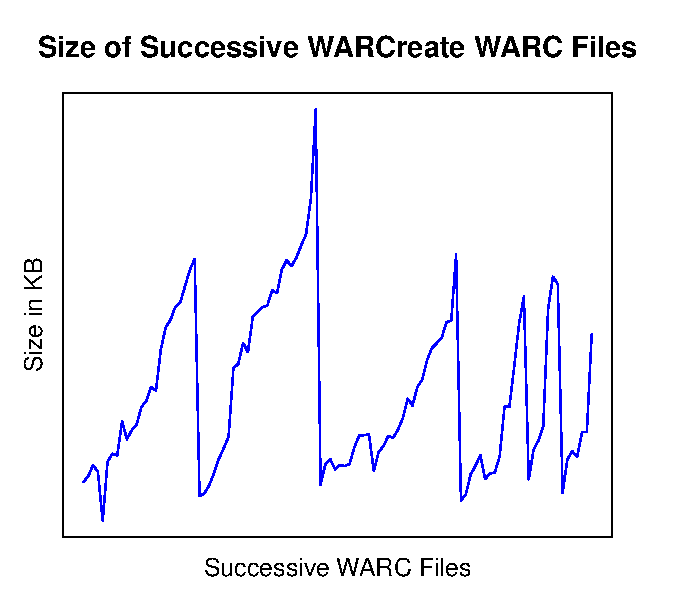
\includegraphics{stats/warcreate_ordered_sizes.pdf}
\end{figure}
Each ``crash'' in the graph corresponds to a restart of the web browser before the next WARC file was
generated. This suggests Successive WARC files are including content from previous WARC files, which
could explain the relatively high average number of requests and responses in the WARCreate WARC files.

\subsection{Playback}
Playback of WARC files was conducted using two tools: the Wayback Machine included in the WAIL utility,
and the ``Replay'' feature of WebRecorder.io. Screen captures of the original webpages for each of three sample
URIs are shown in the Appendix B. The three sample URIs are listed in Appendix A.

Using the Wayback Machine was a bit of a hassle because
I had to be careful to know which set of WARC files were being played-back. There was no clear output of
the source filename, so I decided to only load one set of WARCs into the Wayback Machine at a time. The
Wayback Machine also did not appear to display pages from a gzip compressed WARC file, although it seemed
to index these files correctly. Screen captures of the Wayback Machine's rendering of the sample WARC files
are in the second Appendix C.

WebRecorder.io's Replay feature simply required me to upload each sample WARC file and click the ``Replay''
button. A screen capture of each rendering of the sample WARCS is shown in the third Appendix D.

Overall, both playback tools preformed decently. However, all three sample WARC files produced using
WebRecorder.io failed catastrophically when rendered in the Wayback Machine. The rendered pages appeared to
have a strange encoding composed primarily of characters not displayable by Google Chrome. Other than that
combination of WARC generation and playback tools, everything worked well enough to read any text on the page
except one URI saved by WARCreate would not work at all when replayed using WebRecorder.io

Of the 18 rendered WARC files, 12 displayed correctly with the exception of missing multimedia. Four rendered
WARCs did not display any of the content as the original webpage, and two appeared to be missing stylesheets
and were a chore to read.

\subsection{SOLR Queries}
I made four queries of the SOLR database after I loaded it with all my WARC files created by wget. The first
two queries just test the generic search terms ``linux'' and ``marathon''. The third query searches for only
documents that contain ``linux'' in the document title, as detemrined by SOLR. The fourth query searches only
for documents with the ``keywords'' field set. This field appeared to be populated only in documents that
contained the below HTML tag.
\begin{lstlisting}[basicstyle=\ttfamily,escapechar=@]
    <meta name="keywords" content="@\emph{keyphrases}@"/>
\end{lstlisting}
In the tag, \emph{keyphrases} is a comma-separated list of keywords, that may contain spaces. A common
keyphrase, was ``boston marathon''.

The results of the queries are shown abridged in screen captures in the fourth Appendix E. They are also shown
in complete form in text in my GitHub repository
\footnote{\url{https://github.com/jamesbtate/cs851-s15/tree/master/hw2_report/queries}} for this project.


\clearpage
\begin{appendices}

\section{Sample URIs}
The three below URIs are the ones used when testing rendering WARC files. They are numbered for their
frequency in my list of final URIs in assignment one. URI \#1 was the most frequent URI.
\begin{description}
 \item[1.] \url{https://represent.com/connor}
 \item[6.] \url{http://www.nba.com/kings/news/cousins-2015-allstar}
 \item[23.] \url{https://www.youtube.com/watch?v=UC49bpMs4zk}
\end{description}

\section{Original Webpage Screen Captures}

\begin{figure}[H]
    \centering
    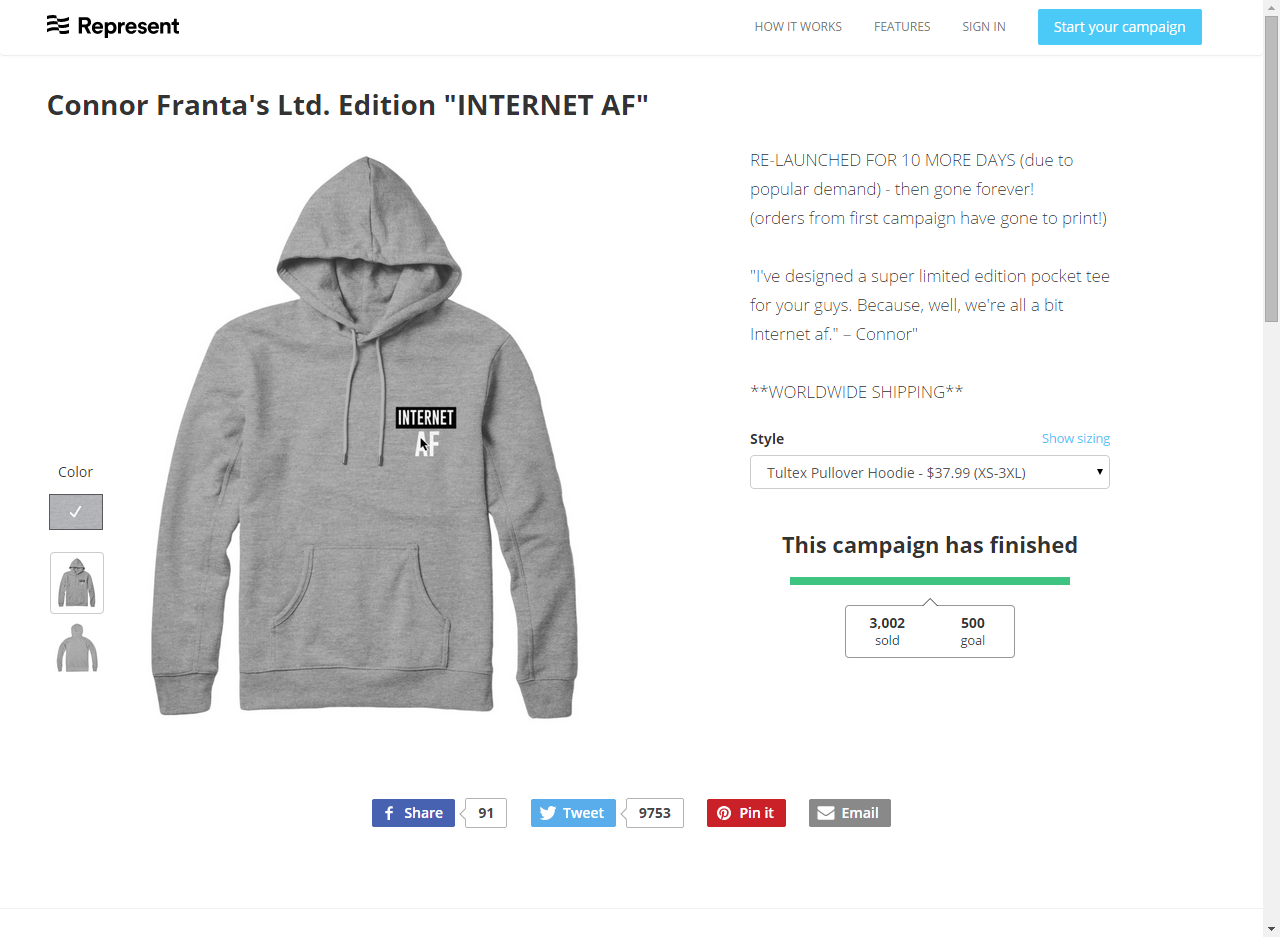
\includegraphics[scale=0.5]{images/1_original.png}
    \caption{Web browser render of representation of URI \#1.}
\end{figure}
\begin{figure}[H]
    \centering
    
\includegraphics[scale=0.5]{images/6_original.png}
    \caption{Web browser render of representation of URI \#6.}
\end{figure}
\begin{figure}[H]
    \centering
    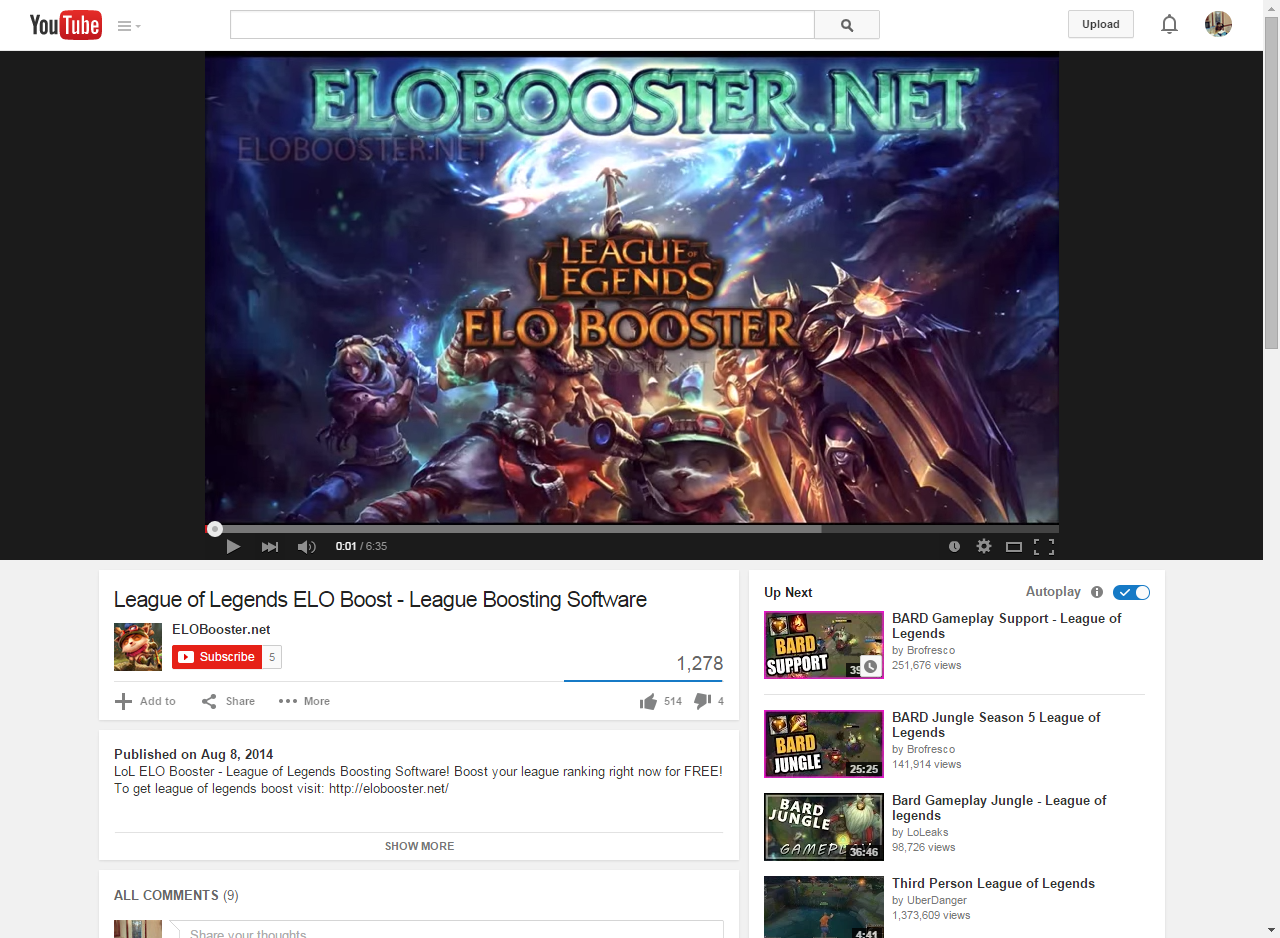
\includegraphics[scale=0.5]{images/23_original.png}
    \caption{Web browser render of representation of URI \#23.}
\end{figure}


\section{Wayback Machine Playback Screen Captures}

\begin{figure}[H]
    \centering
    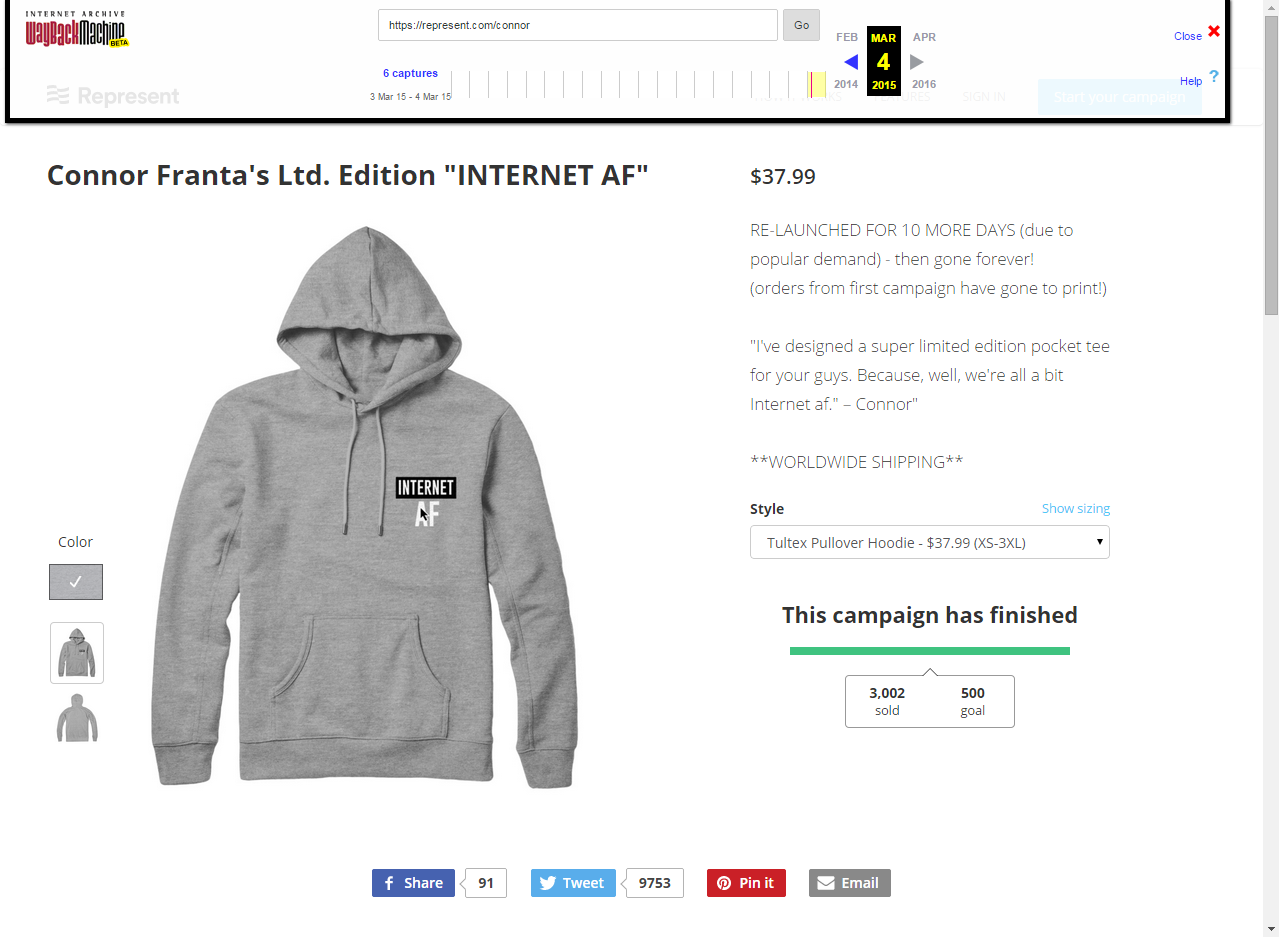
\includegraphics[scale=0.5]{images/1_wget_in_wayback.png}
    \caption{Wayback Machine playback of wget WARC of URI \#1.}
\end{figure}
\begin{figure}[H]
    \centering
    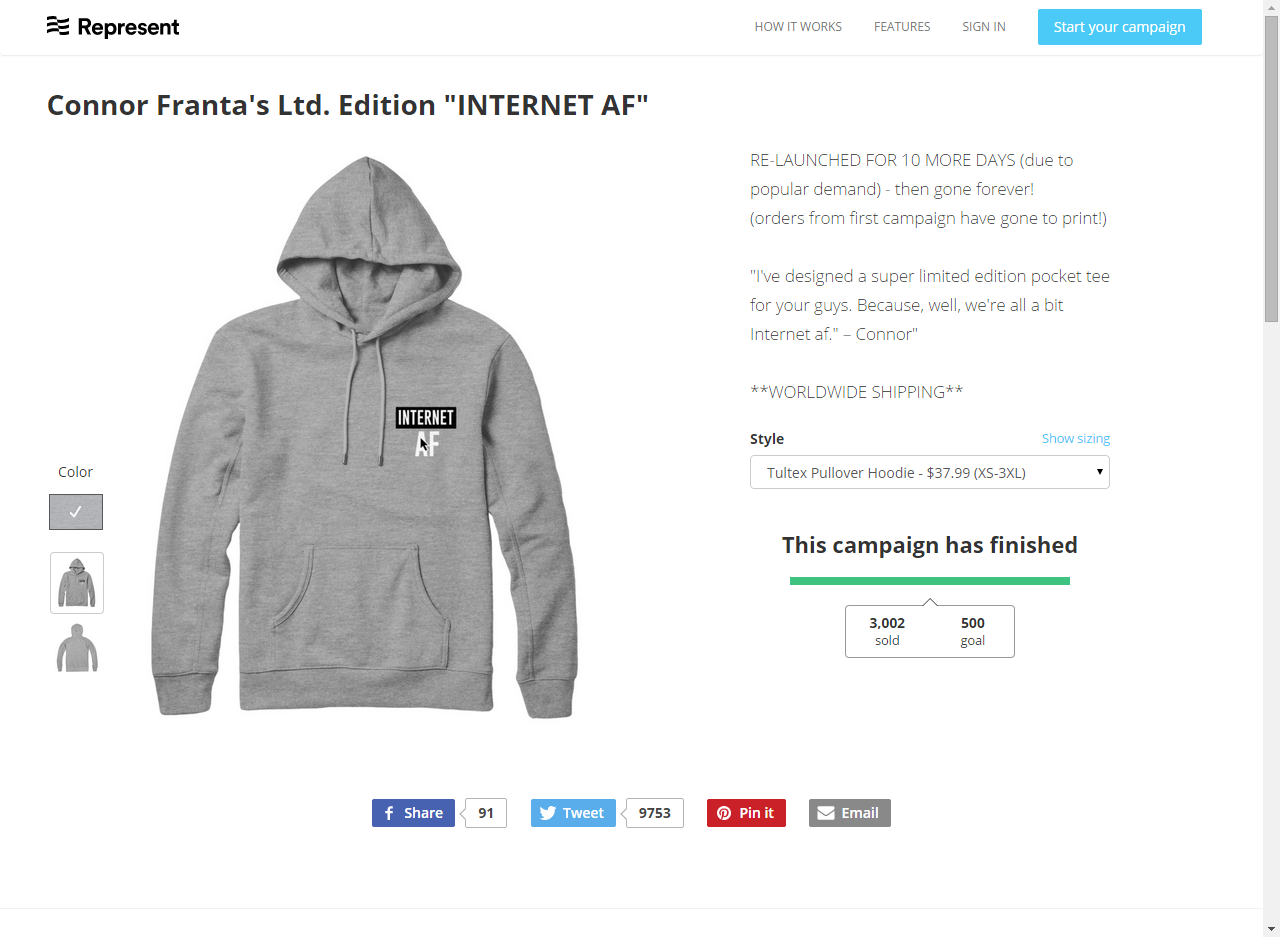
\includegraphics[scale=0.5]{images/1_warcreate_in_wayback.png}
    \caption{Wayback Machine playback of WARCreate WARC of URI \#1.}
\end{figure}
\begin{figure}[H]
    \centering
    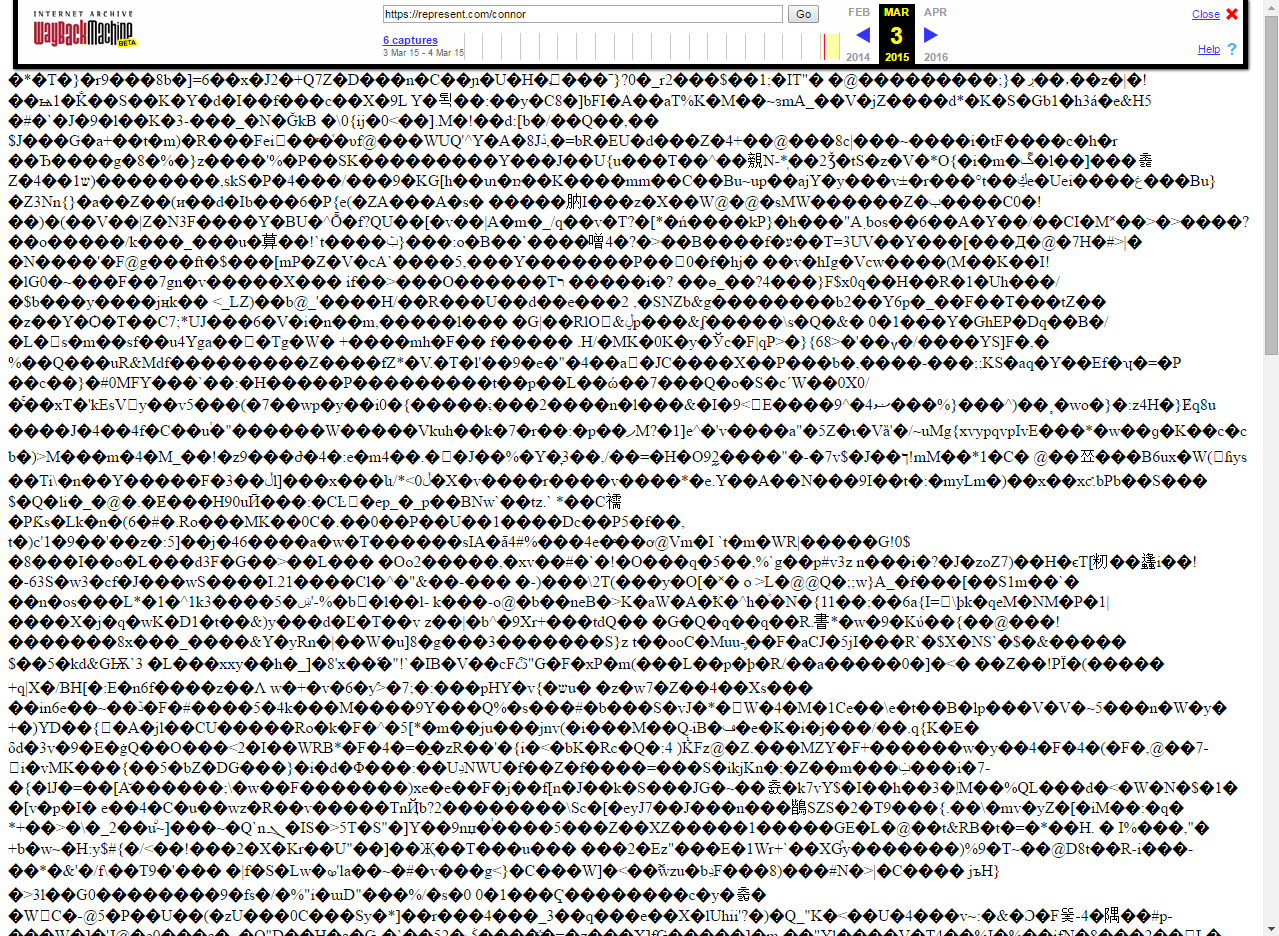
\includegraphics[scale=0.5]{images/1_webrecorder_in_wayback.png}
    \caption{Wayback Machine playback of WebRecorder.io WARC of URI \#1.}
\end{figure}
\begin{figure}[H]
    \centering
    
\includegraphics[scale=0.5]{images/6_wget_in_wayback.png}
    \caption{Wayback Machine playback of wget WARC of URI \#6.}
\end{figure}
\begin{figure}[H]
    \centering
    
\includegraphics[scale=0.5]{images/6_warcreate_in_wayback.png}
    \caption{Wayback Machine playback of WARCreate WARC of URI \#6.}
\end{figure}
\begin{figure}[H]
    \centering
    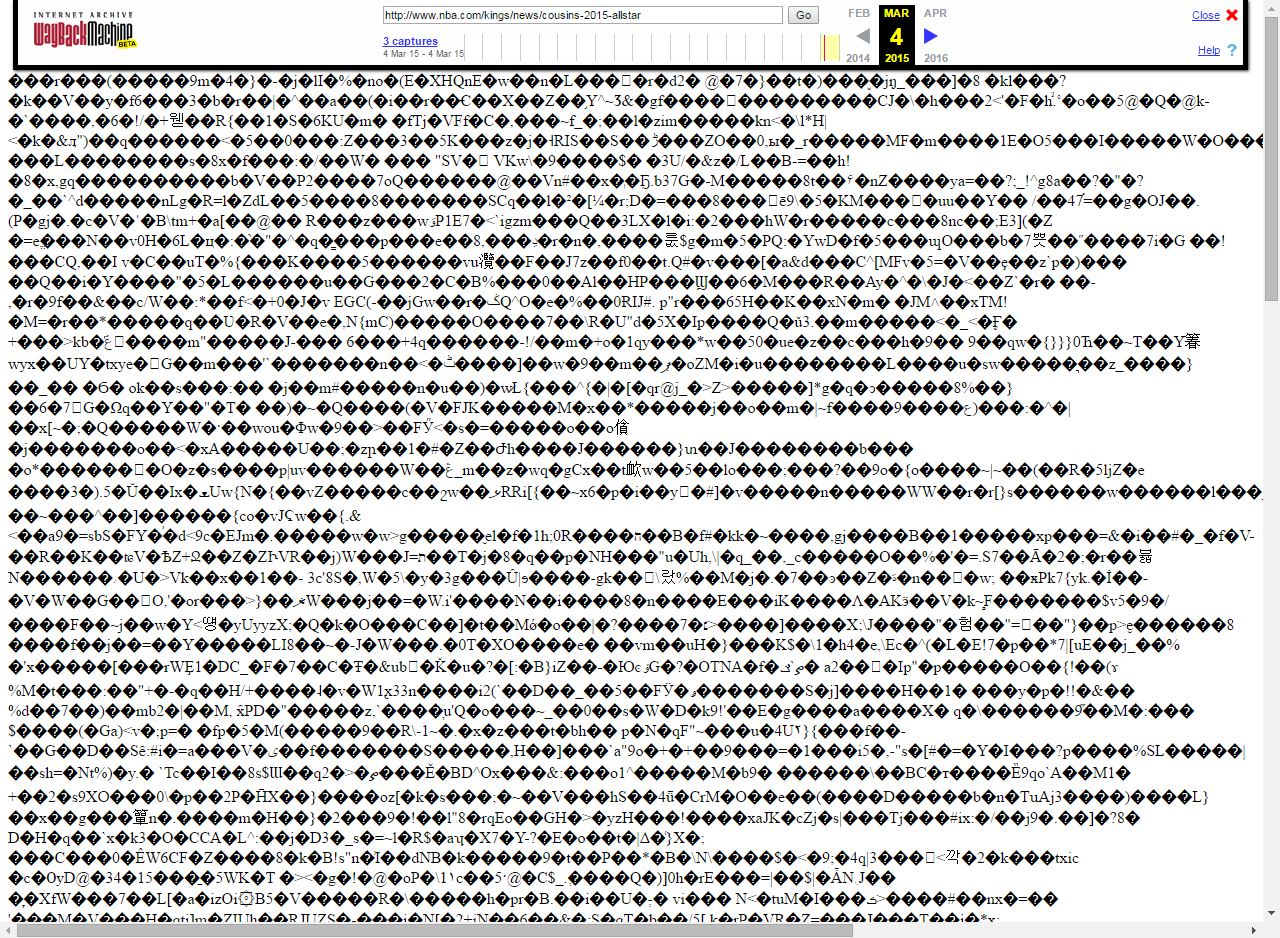
\includegraphics[scale=0.5]{images/6_webrecorder_in_wayback.png}
    \caption{Wayback Machine playback of WebRecorder.io WARC of URI \#6.}
\end{figure}
\begin{figure}[H]
    \centering
    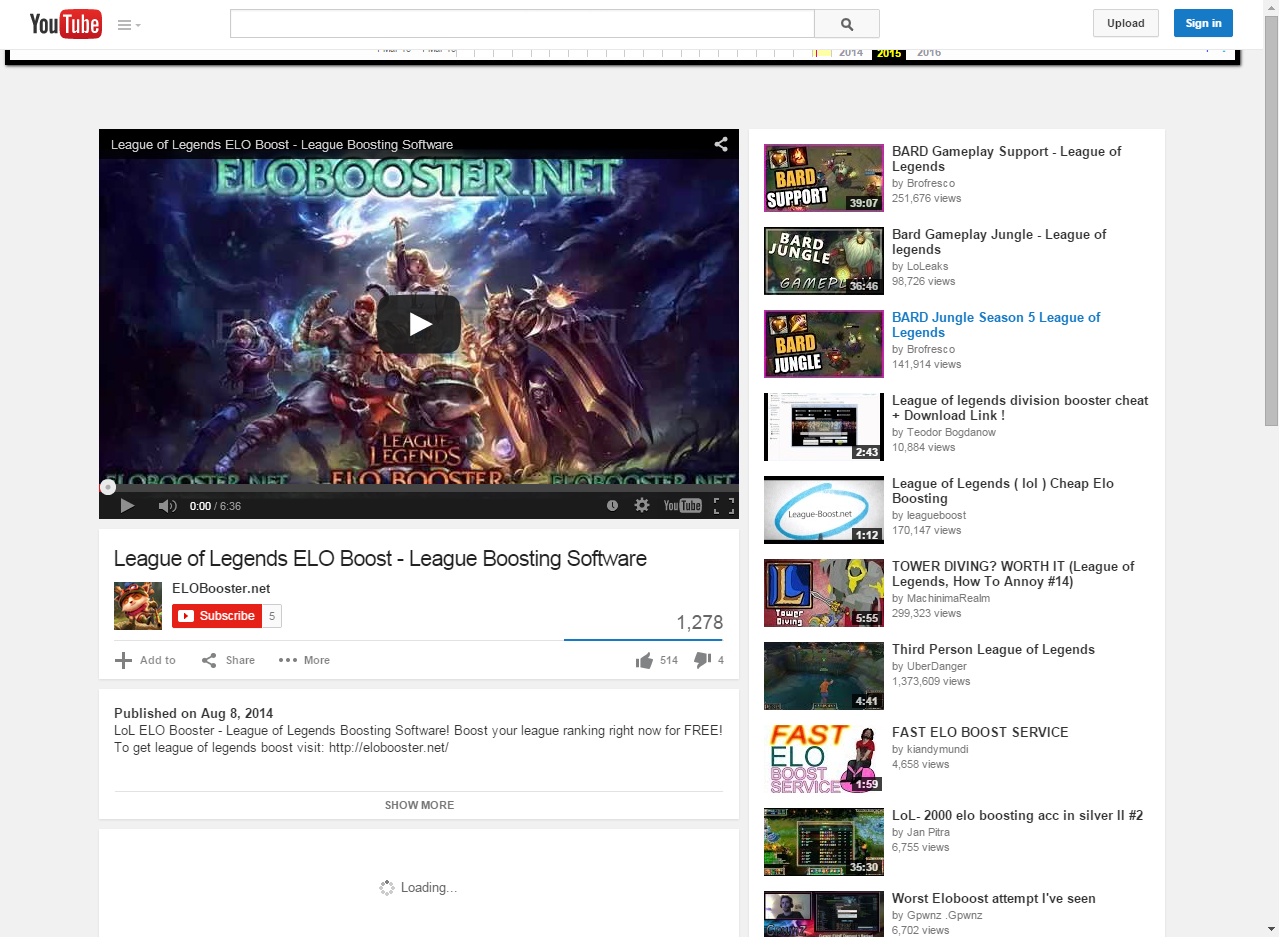
\includegraphics[scale=0.5]{images/23_wget_in_wayback.png}
    \caption{Wayback Machine playback of wget WARC of URI \#23.}
\end{figure}
\begin{figure}[H]
    \centering
    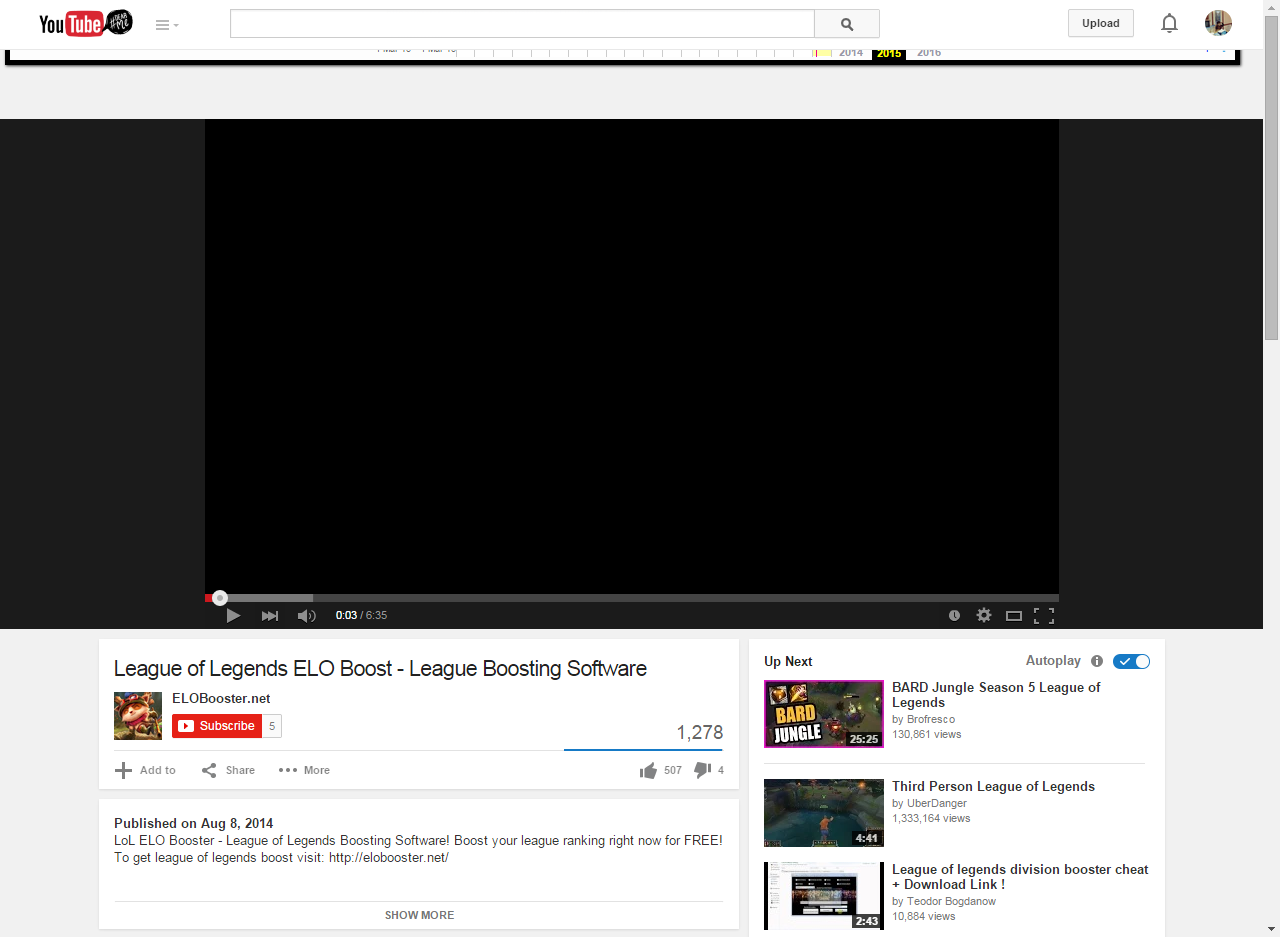
\includegraphics[scale=0.5]{images/23_warcreate_in_wayback.png}
    \caption{Wayback Machine playback of WARCreate WARC of URI \#23.}
\end{figure}
\begin{figure}[H]
    \centering
    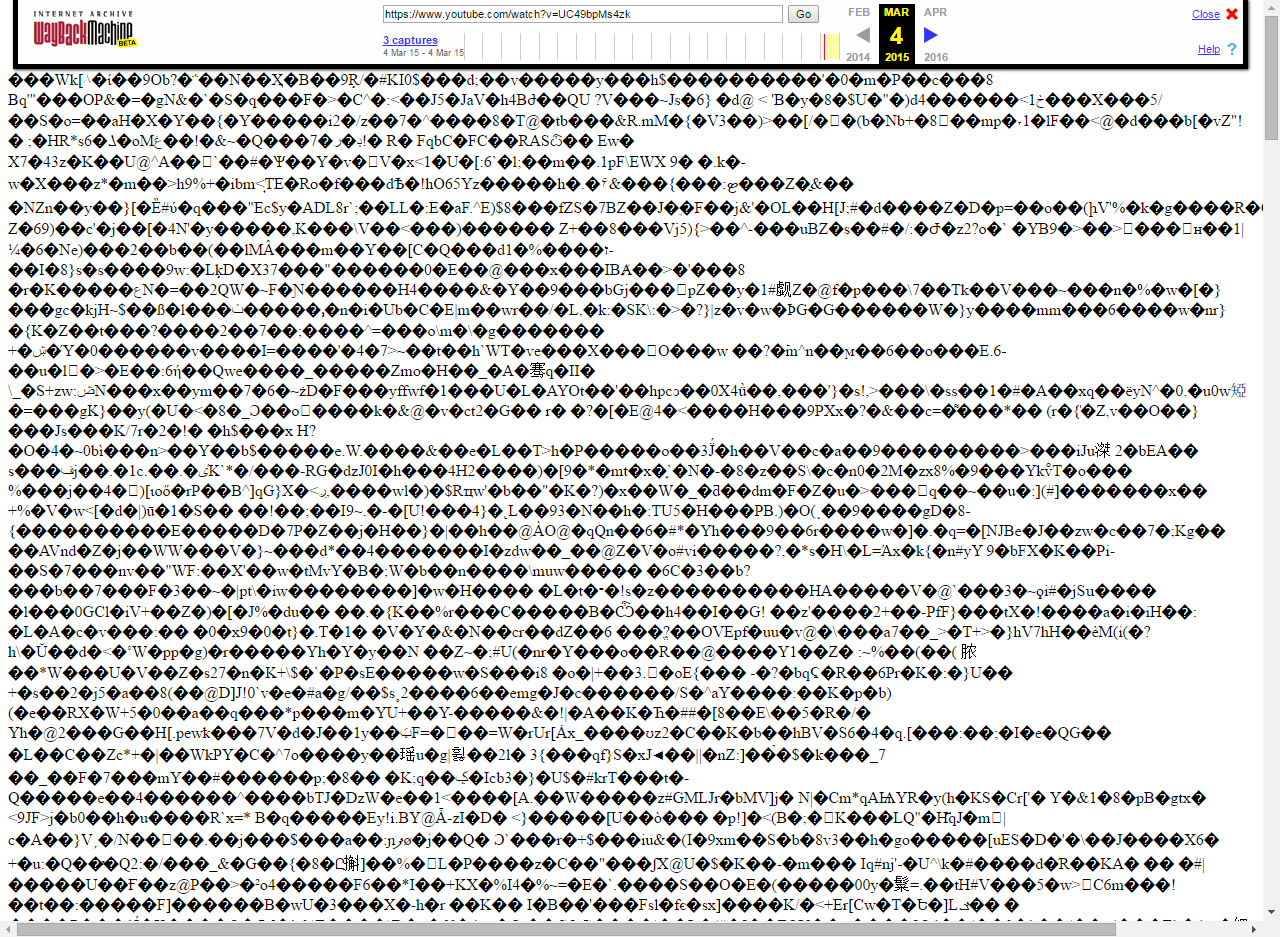
\includegraphics[scale=0.5]{images/23_webrecorder_in_wayback.png}
    \caption{Wayback Machine playback of WebRecorder.io WARC of URI \#23.}
\end{figure}

\section{WebRecorder.io Playback Screen Captures}

\begin{figure}[H]
    \centering
    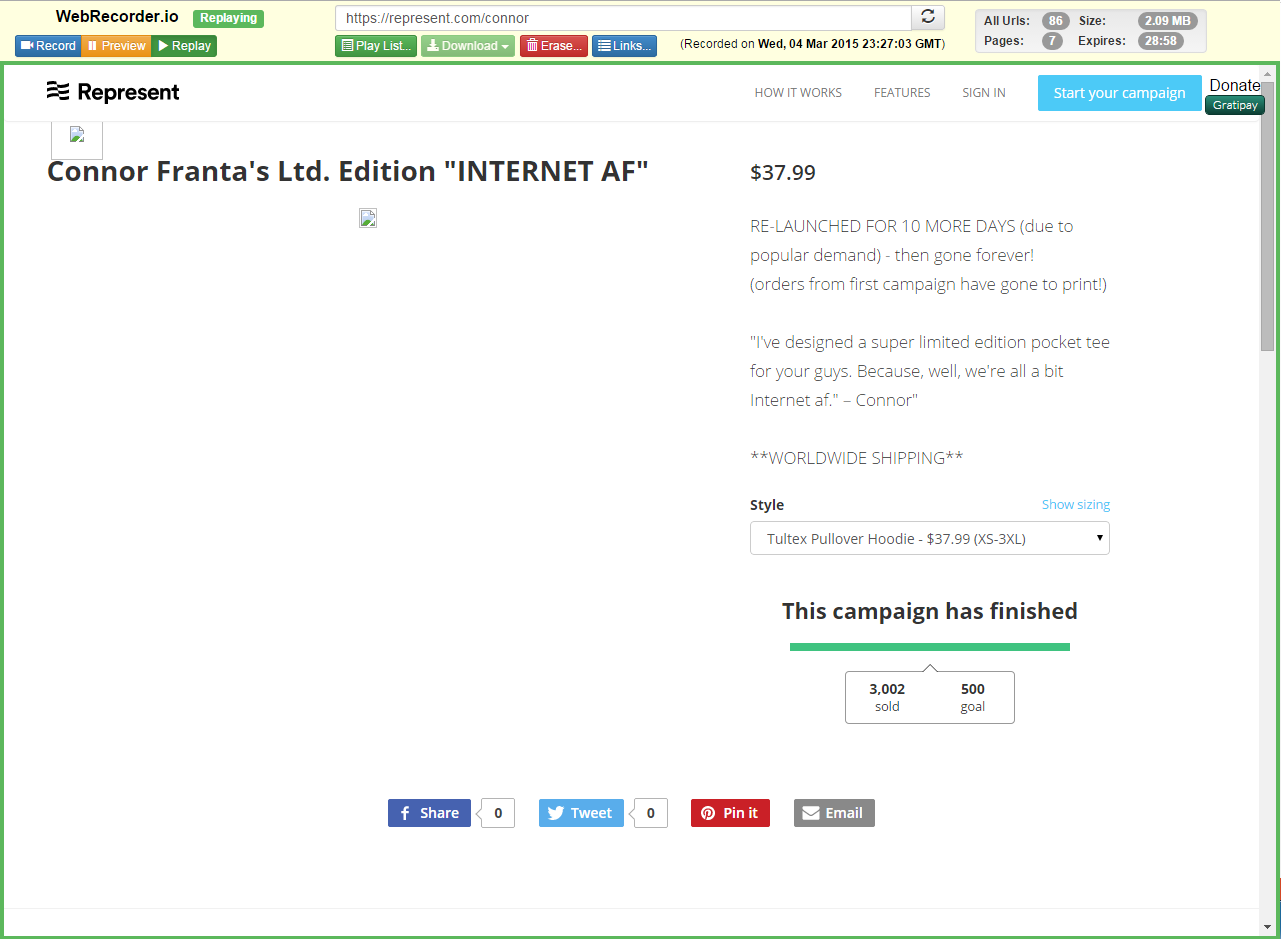
\includegraphics[scale=0.5]{images/1_wget_in_webrecorder.png}
    \caption{WebRecorder.io playback of wget WARC of URI \#1.}
\end{figure}
\begin{figure}[H]
    \centering
    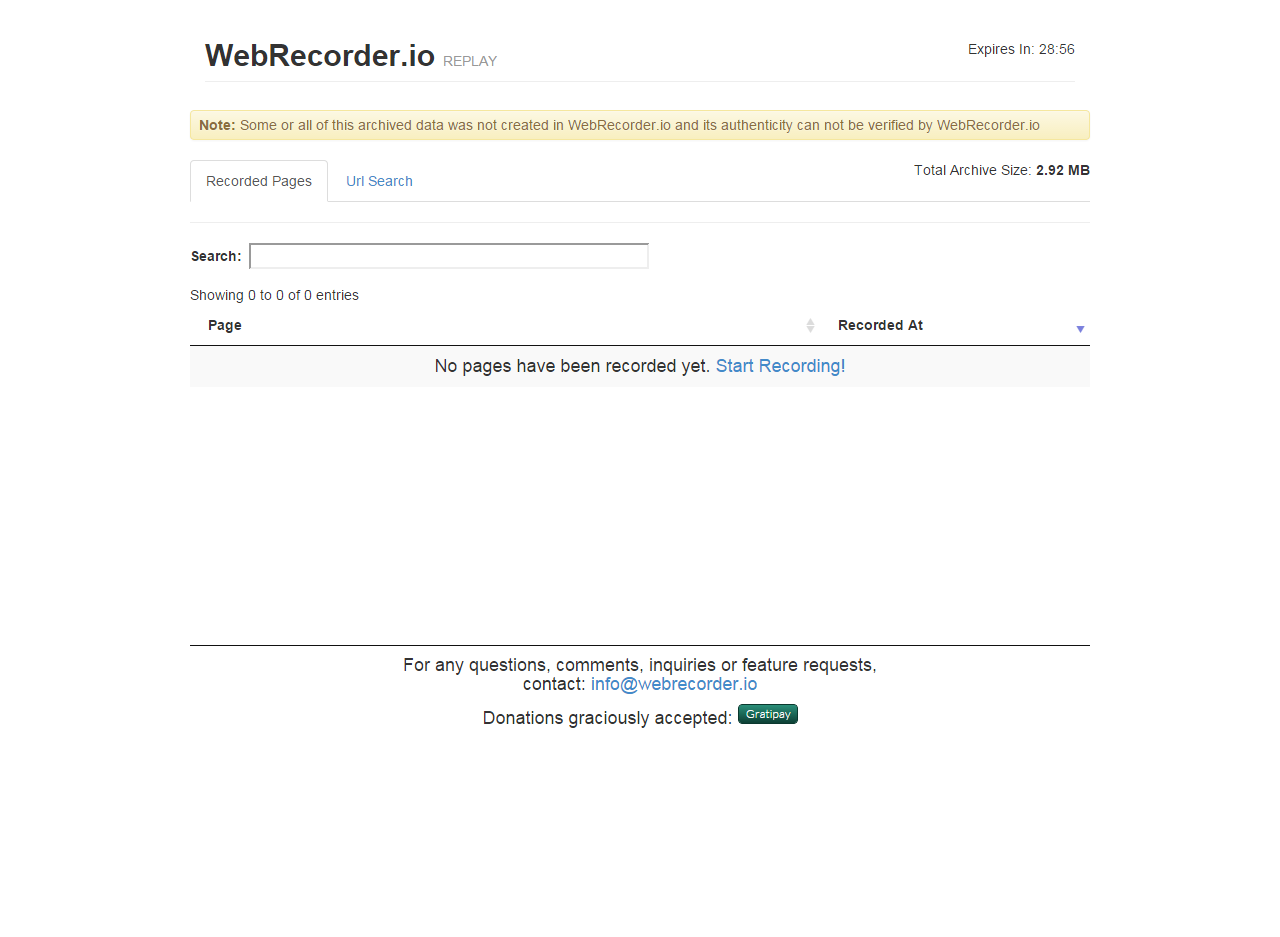
\includegraphics[scale=0.5]{images/1_warcreate_in_webrecorder.png}
    \caption{WebRecorder.io playback of WARCreate WARC of URI \#1.}
\end{figure}
\begin{figure}[H]
    \centering
    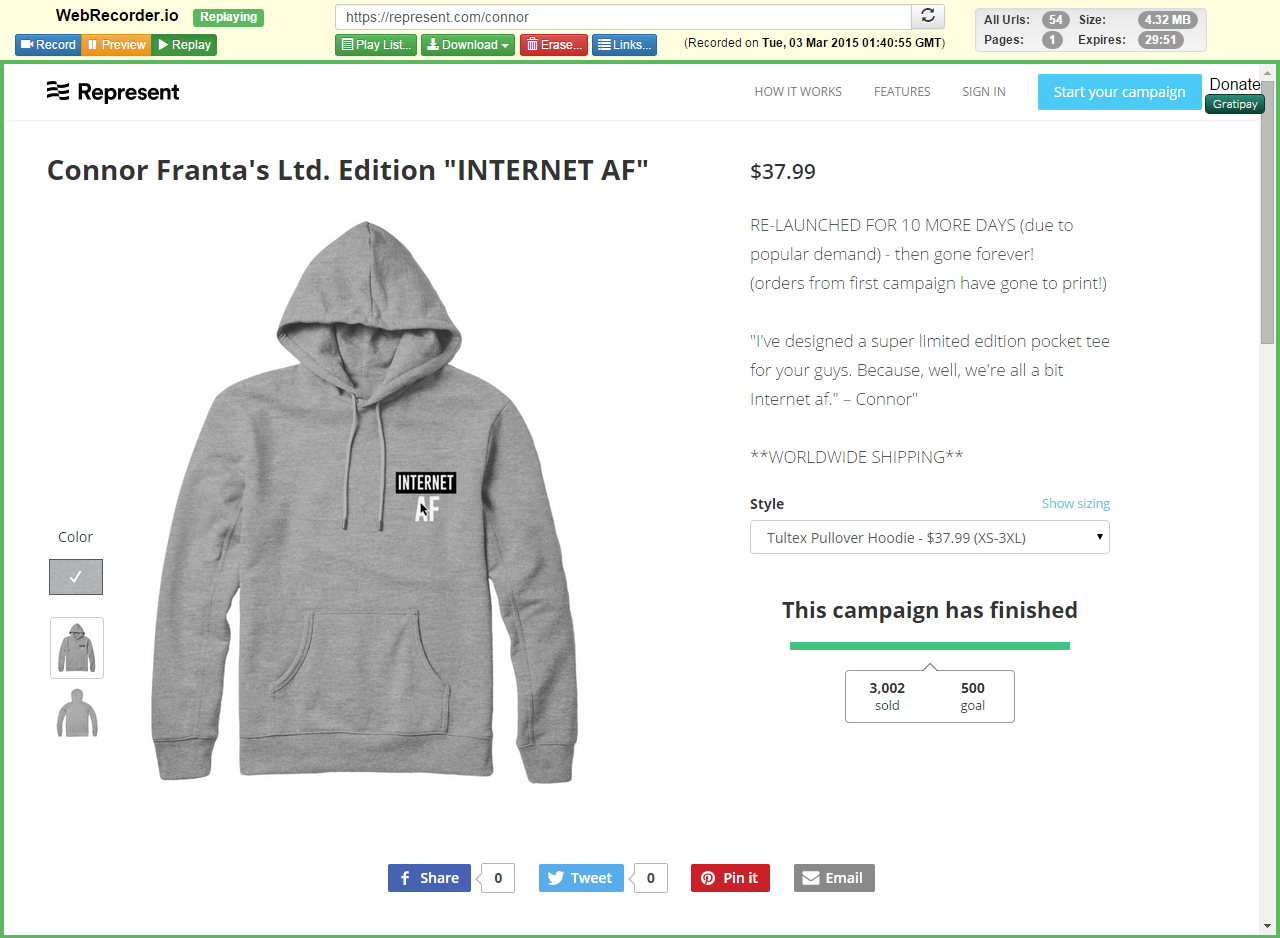
\includegraphics[scale=0.5]{images/1_webrecorder_in_webrecorder.png}
    \caption{WebRecorder.io playback of WebRecorder.io WARC of URI \#1.}
\end{figure}
\begin{figure}[H]
    \centering
    
\includegraphics[scale=0.5]{images/6_wget_in_webrecorder.png}
    \caption{WebRecorder.io playback of wget WARC of URI \#6.}
\end{figure}
\begin{figure}[H]
    \centering
    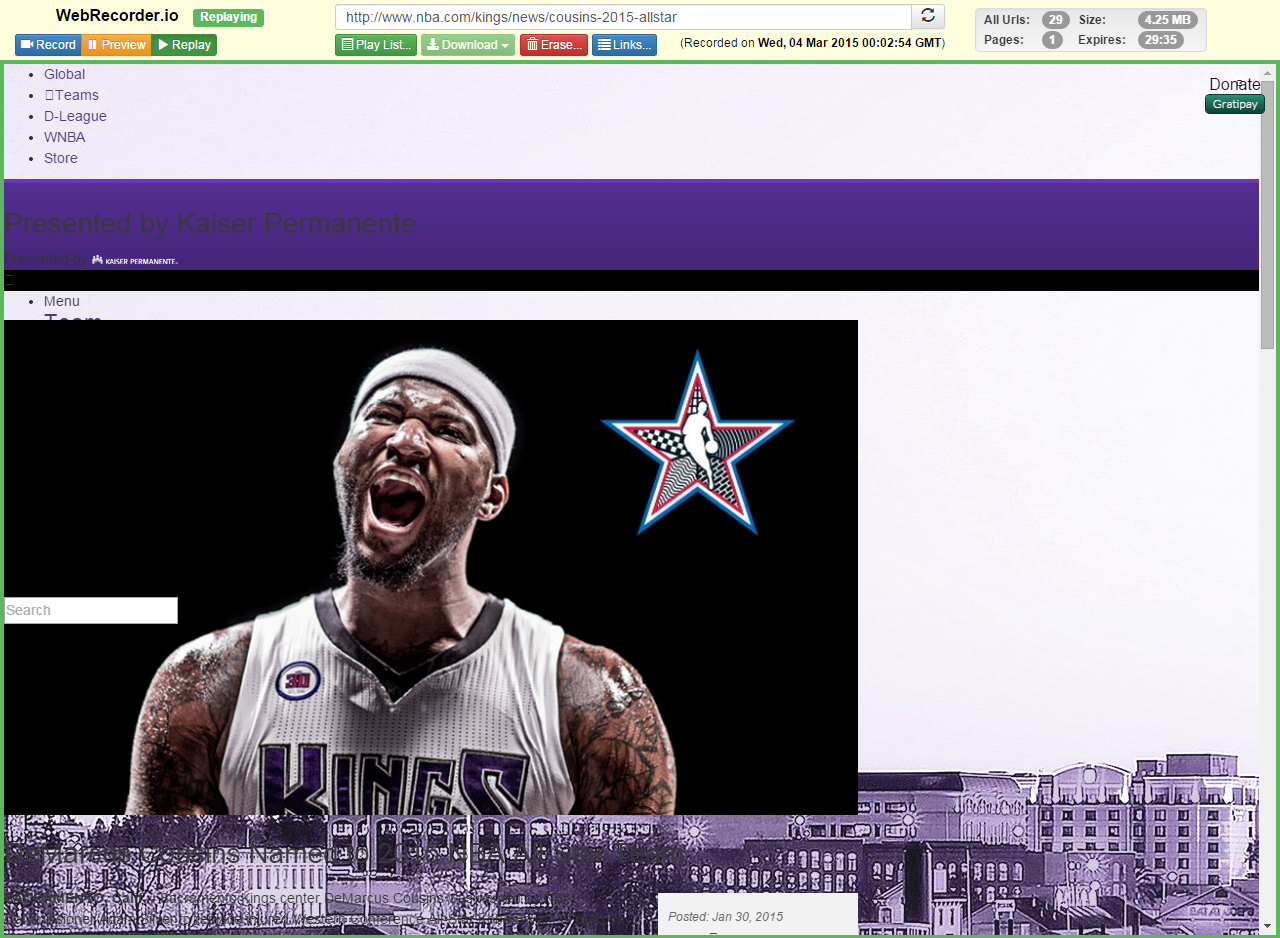
\includegraphics[scale=0.5]{images/6_warcreate_in_webrecorder.png}
    \caption{WebRecorder.io playback of WARCreate WARC of URI \#6.}
\end{figure}
\begin{figure}[H]
    \centering
    
\includegraphics[scale=0.5]{images/6_webrecorder_in_webrecorder.png}
    \caption{WebRecorder.io playback of WebRecorder.io WARC of URI \#6.}
\end{figure}
\begin{figure}[H]
    \centering
    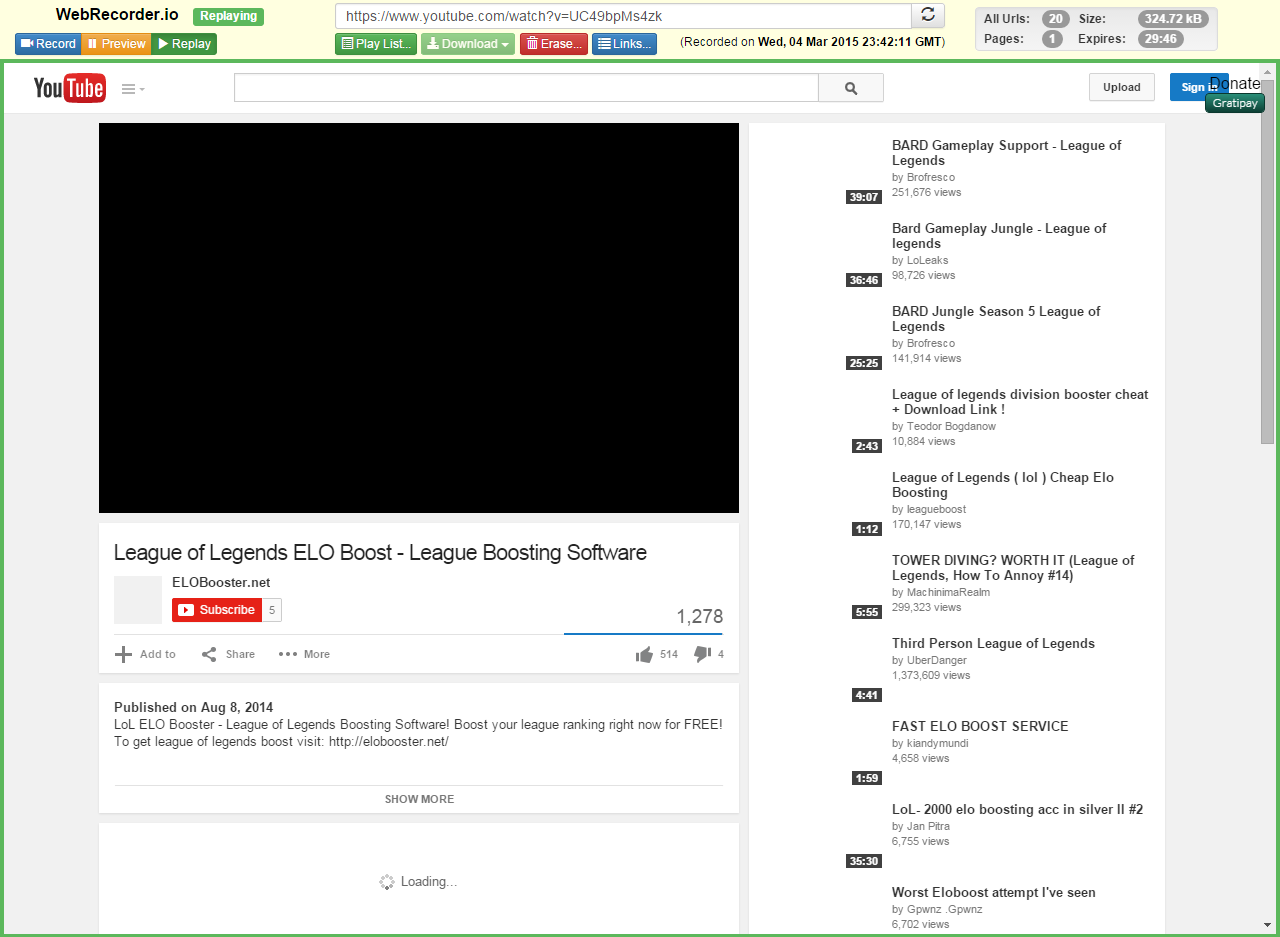
\includegraphics[scale=0.5]{images/23_wget_in_webrecorder.png}
    \caption{WebRecorder.io playback of wget WARC of URI \#23.}
\end{figure}
\begin{figure}[H]
    \centering
    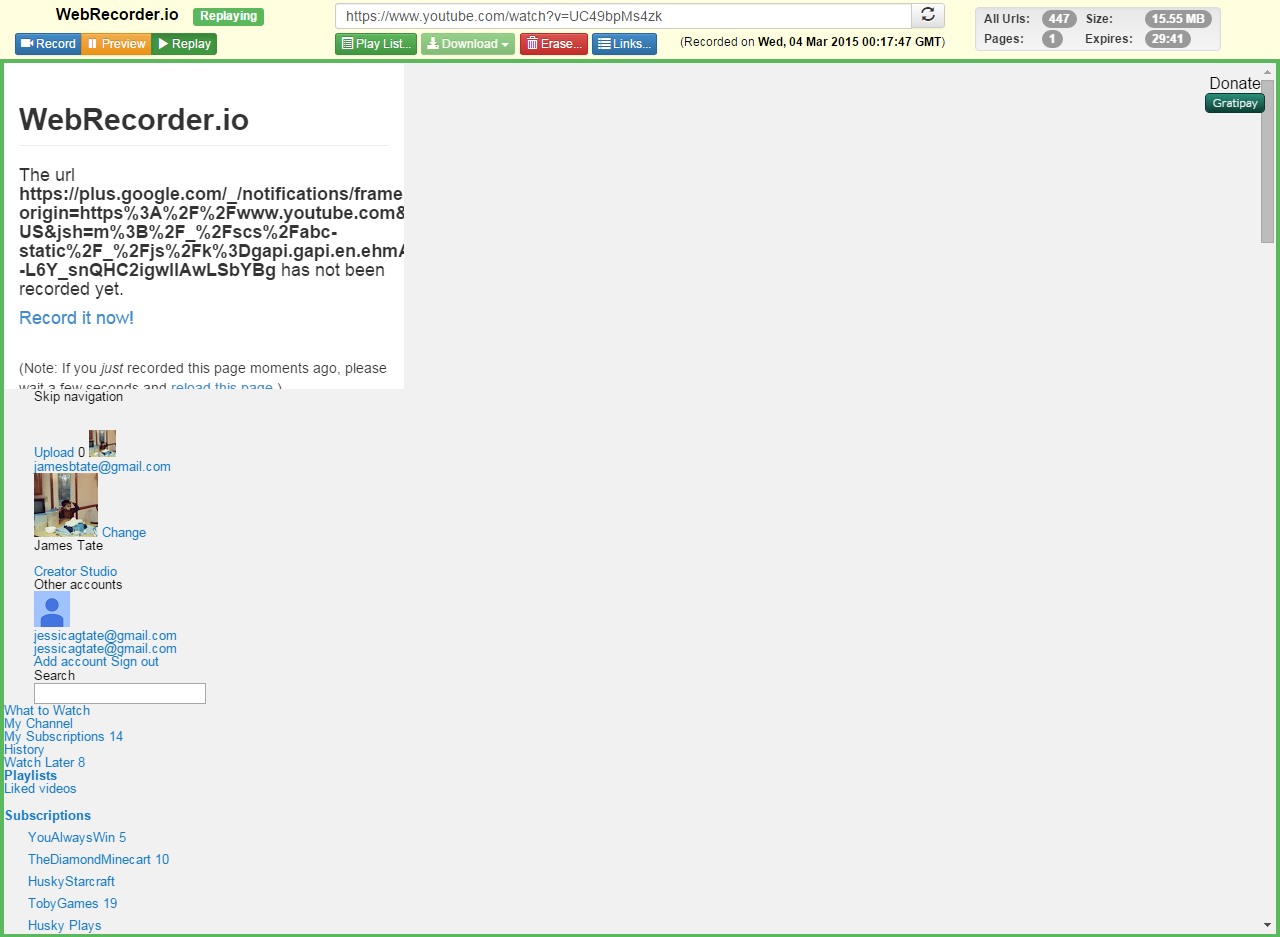
\includegraphics[scale=0.5]{images/23_warcreate_in_webrecorder.png}
    \caption{WebRecorder.io playback of WARCreate WARC of URI \#23.}
\end{figure}
\begin{figure}[H]
    \centering
    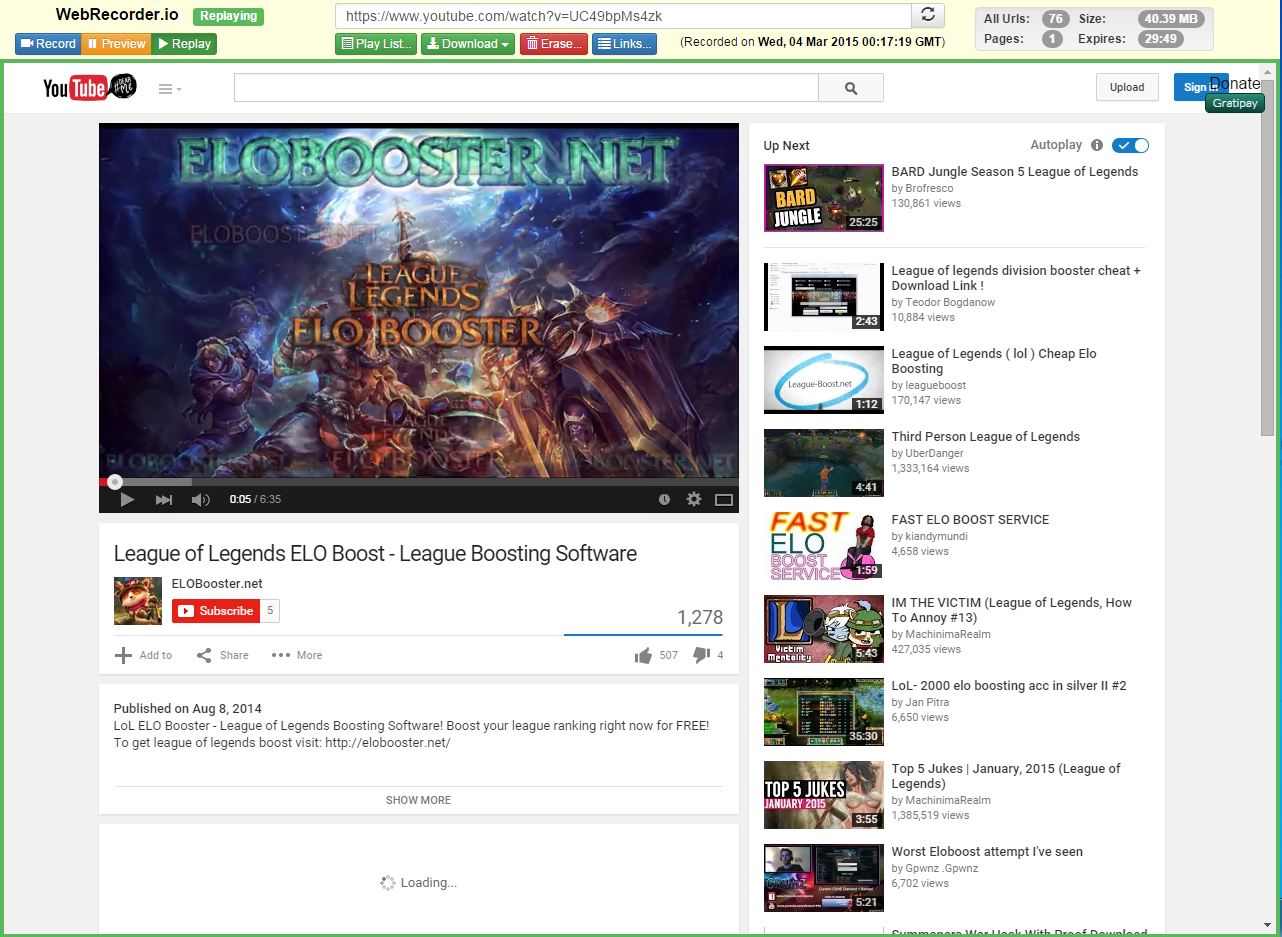
\includegraphics[scale=0.5]{images/23_webrecorder_in_webrecorder.png}
    \caption{WebRecorder.io playback of WebRecorder.io WARC of URI \#23.}
\end{figure}

\section{SOLR Queries}
\begin{figure}[H]
    \centering
    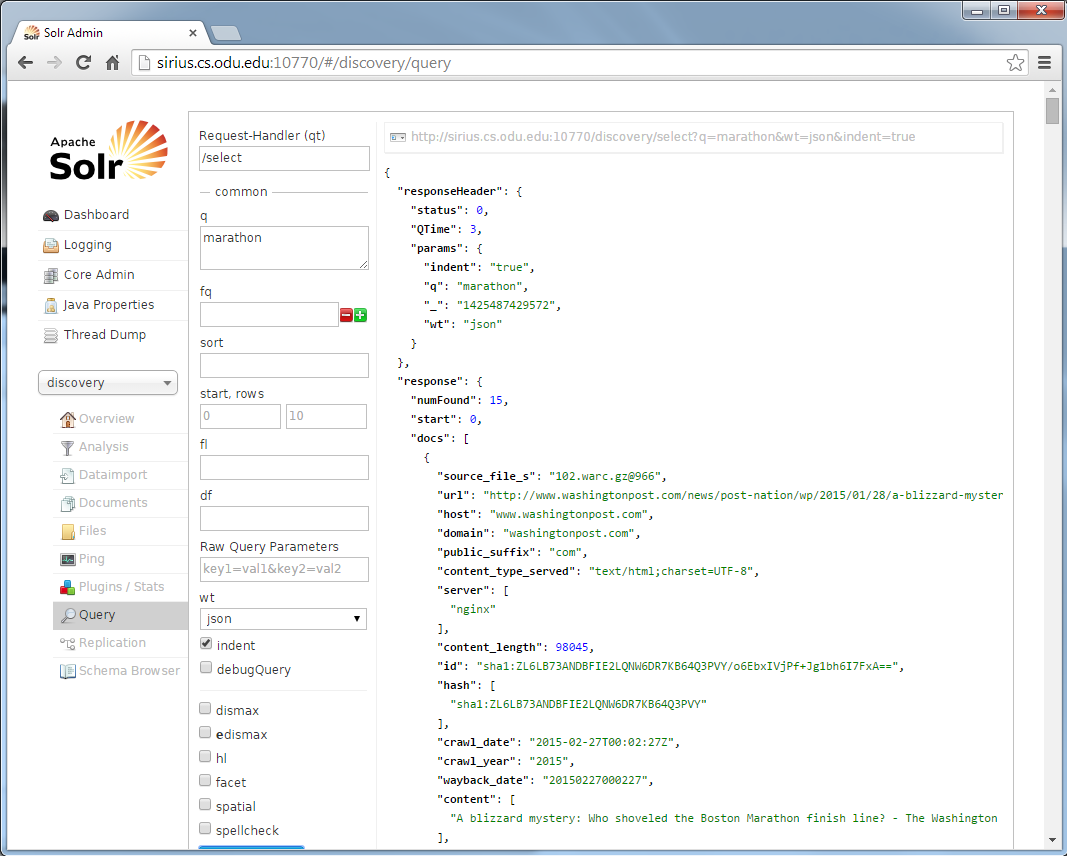
\includegraphics[scale=0.5]{images/query_marathon.png}
    \caption{SOLR query for word ``marathon''.}
\end{figure}
\begin{figure}[H]
    \centering
    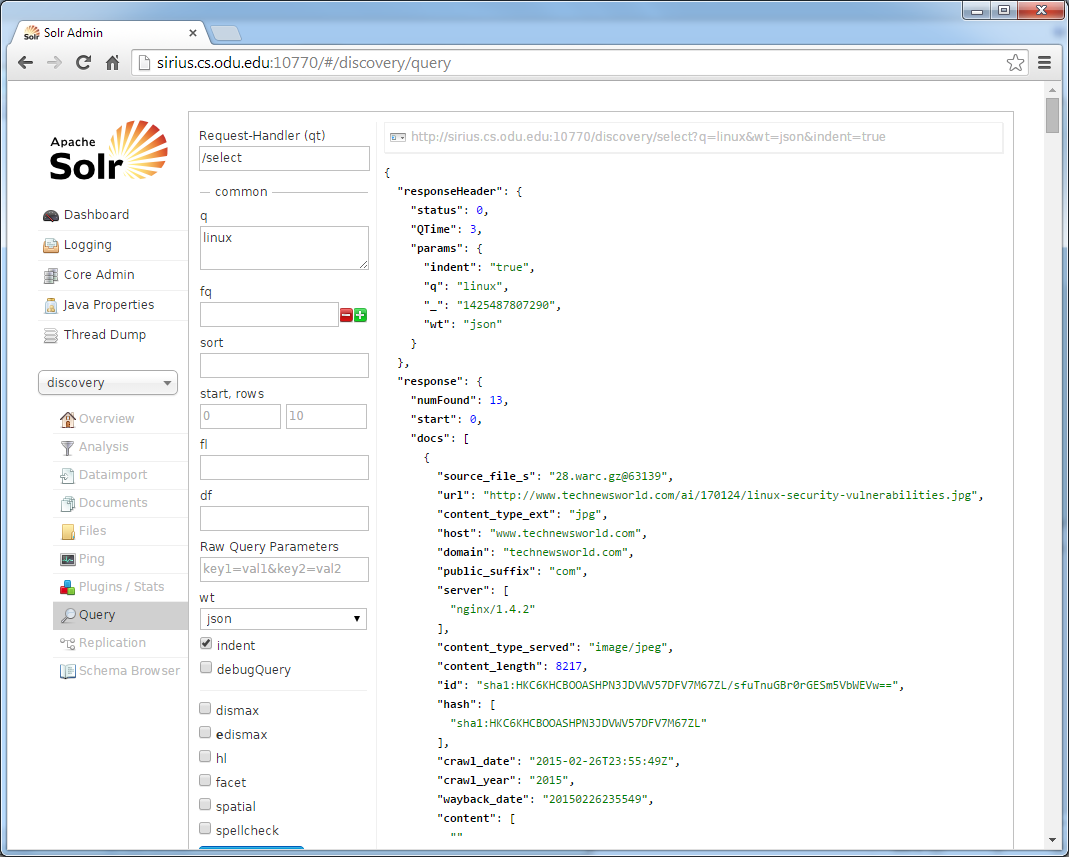
\includegraphics[scale=0.5]{images/query_linux.png}
    \caption{SOLR query for word ``linux''.}
\end{figure}
\begin{figure}[H]
    \centering
    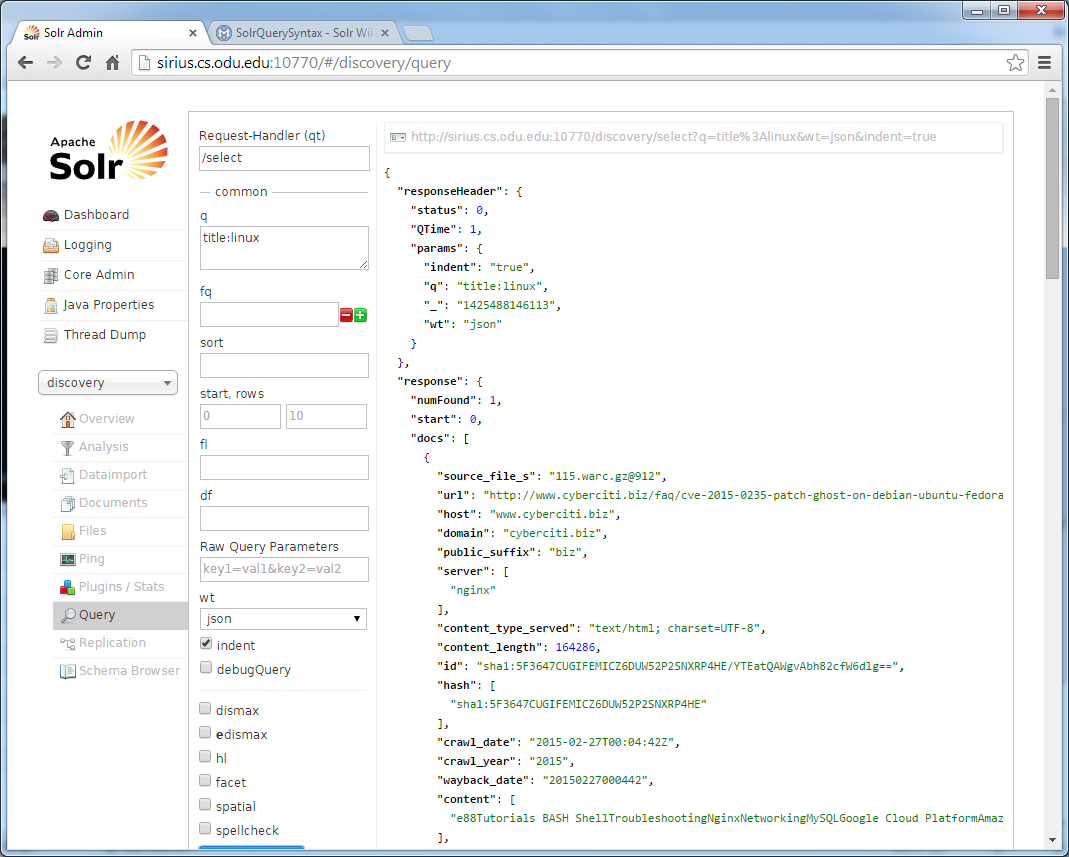
\includegraphics[scale=0.5]{images/query_linux_title.png}
    \caption{SOLR query for documents with ``linux'' in the title.}
\end{figure}
\begin{figure}[H]
    \centering
    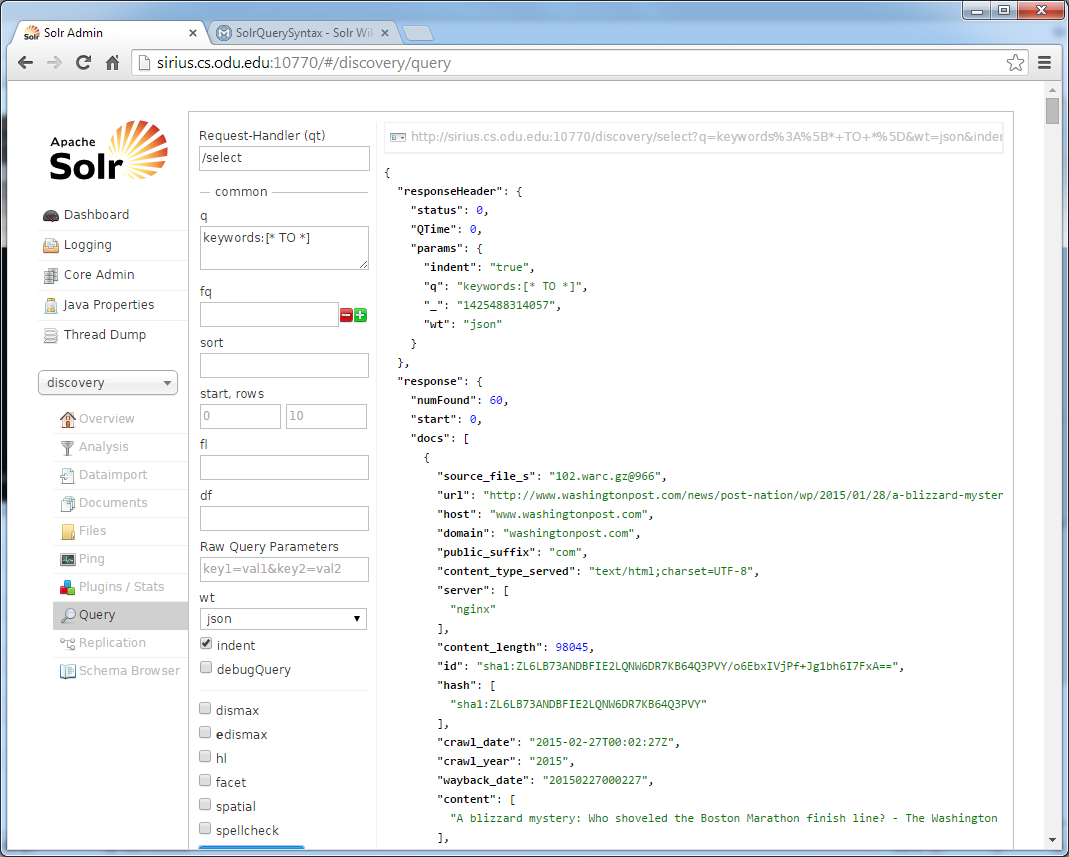
\includegraphics[scale=0.5]{images/query_keywords.png}
    \caption{SOLR query for documents with keyword field set..}
\end{figure}


\end{appendices}

% === no bibliography in this one ===
%\clearpage
%\begin{thebibliography}{9}
%\bibitem{rfc2616}
%    R. Fielding, et. al.,
%    \emph{Hypertext Transfer Protocol -- HTTP/1.1}.
%    \url{https://www.ietf.org/rfc/rfc2616.txt}
%    June 1999.
%\end{thebibliography}

\end{document}
